\documentclass{standalone}

\usepackage{amsmath}
\usepackage{tikz}
\usetikzlibrary{ decorations.markings}
\usetikzlibrary{arrows.meta}

\begin{document}
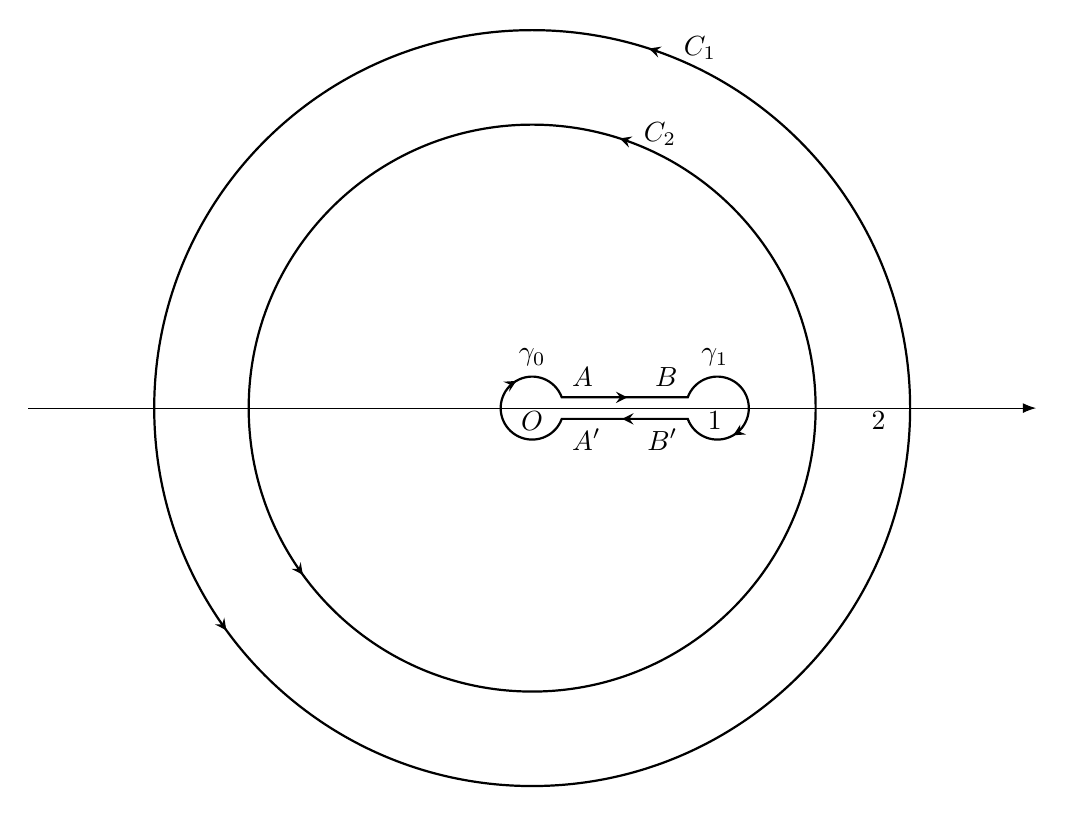
\begin{tikzpicture}[scale=0.8]
    % \draw[help lines] (-7,-7) grid (7,7);
    \draw[thick,postaction={decoration={markings, 
    mark = at position .2 with {\arrow{stealth}},
    mark = at position .6 with {\arrow{stealth}},
    },decorate}] (6,0) arc (0:360:6) --cycle;
    \draw[thick,postaction={decoration={markings, 
    mark = at position .2 with {\arrow{stealth}},
    mark = at position .6 with {\arrow{stealth}},
    },decorate}] (4.5,0) arc (0:360:4.5) --cycle;

    \node at (65:6.3) {$C_1$};
    \node at (65:4.8) {$C_2$};

    \draw[thick,postaction ={decoration={markings,
    mark = at position .2 with {\arrow{stealth}},
    mark = at position .4 with {\arrow{stealth}},
    mark = at position .7 with {\arrow{stealth}},
    mark = at position .9 with {\arrow{stealth}},
    }, decorate}] (-20:0.5) node[below right]{$A'$} arc(-20:-340:0.5) node[above right]{$A$}-- ([xshift=2cm] 20:0.5) node[above left]{$B$} arc(-20:-340:-0.5) node[below left]{$B'$}--cycle;

    \draw[-Latex] (-8,0) -- (8,0) ;
    \node at (0, 0.8) {$\gamma_{0}$};
    \node at (2.9, 0.8) {$\gamma_{1}$};
    \node at (0, -0.2) {$O$};
    \node at (2.9, -0.2) {$1$};
    \node at (5.5, -0.2) {$2$};
\end{tikzpicture}
\end{document}